% \documentclass[12pt, twoside]{article}
\usepackage[letterpaper, margin=1in, headsep=0.2in]{geometry}
\setlength{\headheight}{0.6in}
%\usepackage[english]{babel}
\usepackage[utf8]{inputenc}
\usepackage{microtype}
\usepackage{amsmath}
\usepackage{amssymb}
%\usepackage{amsfonts}
\usepackage[nomessages]{fp} %\FPeval{\var-name}{2*sin(pi/6)}
\usepackage{siunitx} %units in math. eg 20\milli\meter
\usepackage{yhmath} % for arcs, overparenth command
\usepackage{tikz} %graphics
\usetikzlibrary{quotes, angles, arrows, arrows.meta}
\usepackage{graphicx} %consider setting \graphicspath{{images/}}
\usepackage{parskip} %no paragraph indent
\usepackage{enumitem}
\usepackage{multicol}
\usepackage{venndiagram}

\usepackage{fancyhdr}
\pagestyle{fancy}
\fancyhf{}
\renewcommand{\headrulewidth}{0pt} % disable the underline of the header
\raggedbottom
\hfuzz=2mm %suppresses overfull box warnings

\usepackage{hyperref}

\fancyhead[LE]{\thepage}
\fancyhead[RO]{\thepage \\ Name: \hspace{4cm} \,\\}
\fancyhead[LO]{BECA / Dr. Huson / Geometry\\*  Unit 2: Angles\\* 28 Sept 2022}

\begin{document}

\subsubsection*{2.1 Homework: Segment and area review}
\begin{enumerate}
\item Do Now: The horizontal line segment $\overline{RS}$ is plotted on the coordinate plane with $R(2,3)$ and $S(7,3)$. 
  \begin{multicols}{2}
    Find length $RS$, showing the calculation.
      \begin{flushright}
      \begin{tikzpicture}[scale=.635]
        \draw [help lines] (-1,-1) grid (9,6);
        \draw [thick, ->] (-1.2,0) -- (9.4,0) node [below right] {$x$};
        \draw [thick, ->] (0,-1.2)--(0,6.4) node [left] {$y$};
        \draw [-, thick] (2,3)--(7,3);
        \draw [fill] (2,3) circle [radius=0.05] node[below]{$R(2,3)$};
        \draw [fill] (7,3) circle [radius=0.05] node[below right]{$S(7,3)$};
      \end{tikzpicture}
      \end{flushright}
  \end{multicols} 

\item The vertical line segment $\overline{PQ}$ is plotted on the coordinate plane with $P(3,5)$ and $Q(3,1)$. 
  \begin{multicols}{2}
    Find the length $PQ$. \\[0.5cm]
    Show the calculation, including the absolute value bars.
      \begin{flushright}
      \begin{tikzpicture}[scale=.635]
        %\draw [help lines] (-1,-1) grid (9,9);
        \draw [thick, ->] (-1.2,0) -- (9.4,0) node [below right] {$x$};
        \draw [thick, ->] (0,-1.2)--(0,7.4) node [left] {$y$};
        \draw [-, thick] (3,5)--(3,1);
        \draw [fill] (3,5) circle [radius=0.05] node[right]{$P(3,5)$};
        \draw [fill] (3,1) circle [radius=0.05] node[right]{$Q(3,1)$};
      \end{tikzpicture}
      \end{flushright}
  \end{multicols}

\begin{multicols*}{2}
\item Given $\overline{ABC}$, $AB=84$, $AC=116$.\\ [0.25cm]
  Find ${BC}$.\\[1.5cm]
  \begin{tikzpicture}
    \draw [-, thick] (1,0)--(7,0);
    \draw [fill] (1,0) circle [radius=0.05] node[below]{$A$};
    \draw [fill] (5,0) circle [radius=0.05] node[below]{$B$};
    \draw [fill] (7,0) circle [radius=0.05] node[below]{$C$};
  \end{tikzpicture} \vspace{2cm}
\columnbreak

\item Given $\overline{DEF}$, $DE=3 \frac{1}{3}$, and $EF=4 \frac{1}{6}$. \\ [0.25cm]
  Find ${DF}$.\\[1.5cm]
    \begin{tikzpicture}[scale=0.8]
      \draw [-, thick] (0,0)--(7,0);
      \draw [fill] (0,0) circle [radius=0.05] node[below]{$D$};
      \draw [fill] (3,0) circle [radius=0.05] node[below]{$E$};
      \draw [fill] (7,0) circle [radius=0.05] node[below]{$F$};
    \end{tikzpicture} \vspace{2cm}
  \end{multicols*}

\item Given $\overleftrightarrow{PQ}$ as shown on the number line. Find $PQ$. \\[20pt] % Midpoint
  \begin{tikzpicture}
    \draw [<->] (-4.5,0)--(6.5,0);
    \foreach \x in {-4,...,6} %2 leading for diff!=1
      \draw[shift={(\x,0)},color=black] (0pt,-3pt) -- (0pt,3pt) node[below=5pt]  {$\x$};
      \draw [fill] (-2,0) circle [radius=0.05] node[above] {$P$};
      \draw [fill] (4,0) circle [radius=0.05] node[above] {$Q$};
  \end{tikzpicture} \\ \bigskip
  \vspace{1cm}  
  
\item Given $\overleftrightarrow{RS}$, with $R=0.7$ and $S=5.3$. Find $RS$, showing the formula.\\[20pt]
    \begin{tikzpicture}
      \draw [<->] (-4.5,0)--(6.5,0);
      \foreach \x in {-4,...,6} %2 leading for diff!=1
        \draw[shift={(\x,0)},color=black] (0pt,-3pt) -- (0pt,3pt) node[below=5pt]  {$\x$};
        \draw [fill] (0.7,0) circle [radius=0.05] node[above] {$R$};
        \draw [fill] (5.3,0) circle [radius=0.05] node[above] {$S$};
    \end{tikzpicture} \\ \bigskip

\item The shape shown below is composed of straight lines and right angles, with some lengths as marked. Find the perimeter of the figure. Show your work.
  \begin{flushright}
  \begin{tikzpicture}[scale=0.5]
    \draw [-, thick] (0,0)--(13,0)--(13,3)--(9,3)--(9,7)--(13,7)--
    (13, 9)--(0,9)--(0,7)--(4,7)--(4,3)--(0,3)--cycle;
    %\draw [fill] (0,0) circle [radius=0.05] node[left]{$A$};
    %\draw [fill] (7,0) circle [radius=0.05] node[right]{$B$};
    %\draw [fill] (7,2) circle [radius=0.05] node[right]{$C$};
    %\draw [fill] (0,2) circle [radius=0.05] node[left]{$D$};
    \node at (4.5, 5){3};
    \node at (2, 2.5){3};
    \node at (8.5, 5){3};
    \node at (11, 2.5){3};
    \node at (6.5, -0.5){10};
    \node at (13.5, 1.5){2};
    \node at (13.5, 8){1};
  \end{tikzpicture}
  \end{flushright} 

\item Given $\overline{DEFG}$, $DE=1 \frac{2}{5}$, $EF=2 \frac{3}{10}$, and $FG= \frac{4}{5}$. (diagram not to scale)\\ [0.25cm]
  Find ${DG}$, expressed as a fraction, not a decimal.
  \begin{flushright}
    \begin{tikzpicture}
      \draw [-, thick] (0,0)--(9,0);
      \draw [fill] (0,0) circle [radius=0.05] node[below]{$D$};
      \draw [fill] (3,0) circle [radius=0.05] node[below]{$E$};
      \draw [fill] (7,0) circle [radius=0.05] node[below]{$F$};
      \draw [fill] (9,0) circle [radius=0.05] node[below]{$G$};
    \end{tikzpicture}
    \end{flushright}

\item Given the rectangle $ABCD$ shown below, with $AB=6 \frac{1}{3}$ and $BC=2 \frac{1}{2}$. Find the area of the rectangle, expressing your result as a fraction.
  \begin{flushright}
  \begin{tikzpicture}[scale=1.25]
    \draw [-, thick] (0,0)--(4.5,0)--(4.5,2)--(0,2)--cycle;
    \draw [fill] (0,0) circle [radius=0.05] node[left]{$A$};
    \draw [fill] (4.5,0) circle [radius=0.05] node[right]{$B$};
    \draw [fill] (4.5,2) circle [radius=0.05] node[right]{$C$};
    \draw [fill] (0,2) circle [radius=0.05] node[left]{$D$};
    \node at (5, 1){$2 \frac{1}{2}$};
    \node at (2.25, -0.5){$6 \frac{1}{3}$};
  \end{tikzpicture}
  \end{flushright} \vspace{2cm}  

\end{enumerate}
\end{document}